\section{Введение}

\subsection{Актуальность исследования}

\begin{frame}
	\frametitle{Шагающие роботы}
	    \begin{minipage}[t]{0.47\linewidth}
		\textbf{Четырёхногий робот Unitree A1}
		\center{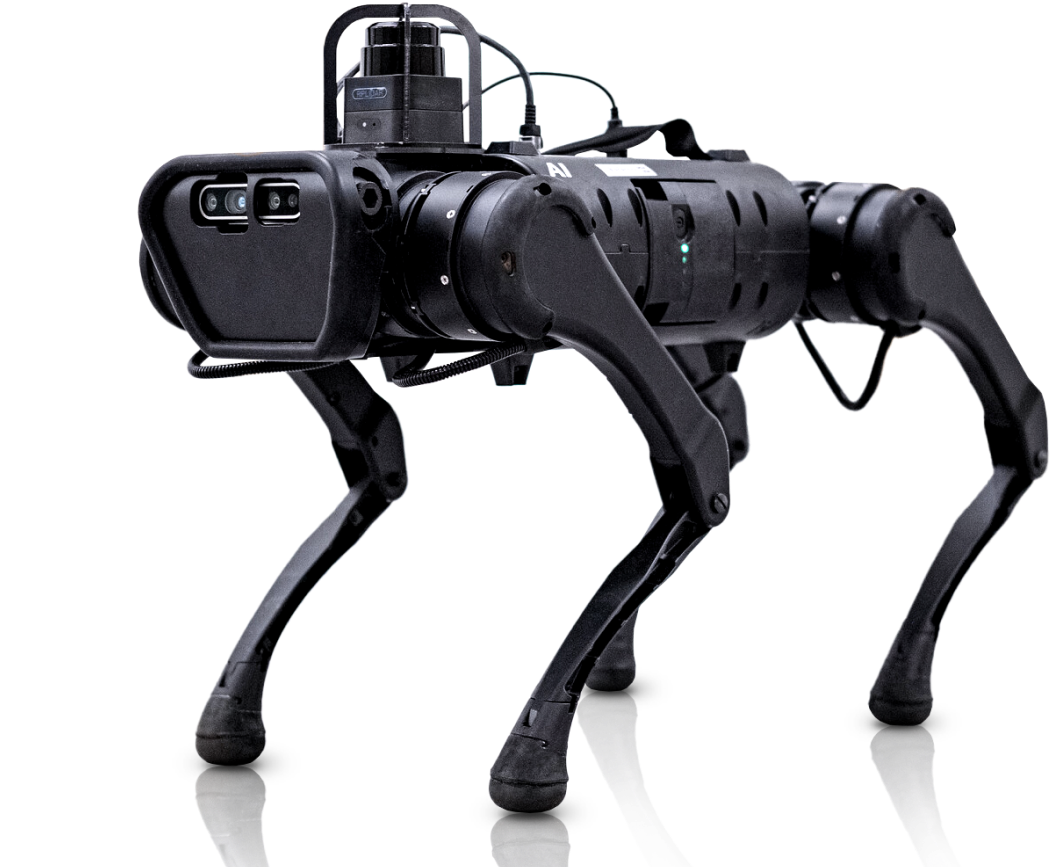
\includegraphics[width=1\linewidth]{images/unitree.png}}
	\end{minipage}
	\hfill
	\begin{minipage}[t]{0.47\linewidth}
		\textbf{Составная \\ подпись 2}
		
	\end{minipage}
\end{frame}

\begin{frame}
    \frametitle{Управление шагающими роботами}
    \centering
	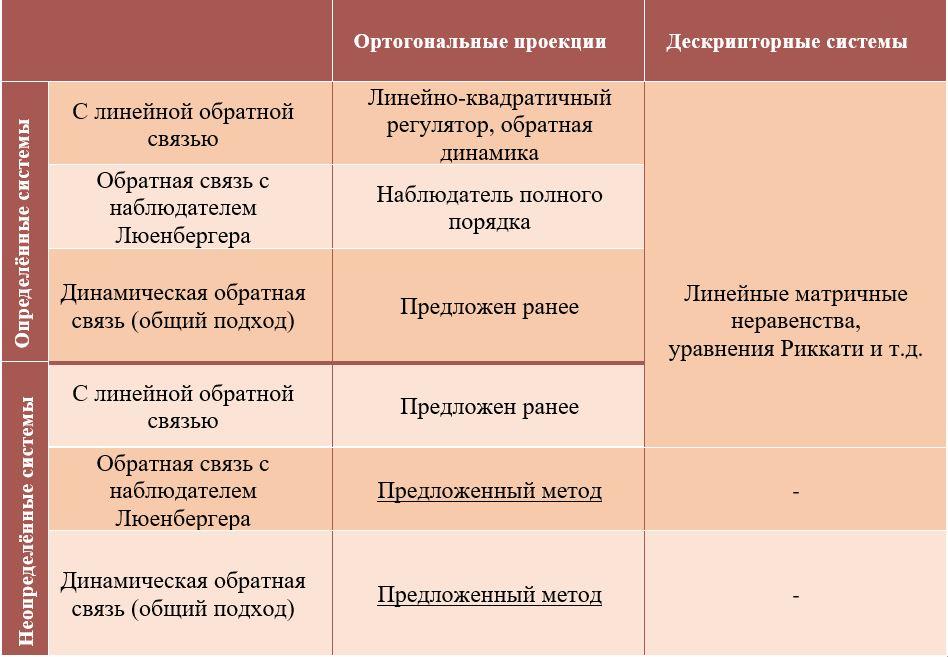
\includegraphics[width=0.85\linewidth]{images/table.JPG} % окружение figure не требуется
\end{frame}

\subsection{Область исследования}

\begin{frame}
    \frametitle{Предмет и объект исследования}
	Объектом исследования является оптимальное робастное управление шагающими роботами с параметрическими неопределённостями.
	\vfill
	Предметом исследования являются методы математического моделирования системы с неопределённостями, описывающие динамику шагающего робота и численные методы с использованием ортогональных методов и линейных матричных неравенств для нахождения коэффициентов регулятора и наблюдателя с последующими вычислениями при помощи комплекса программ.
\end{frame}

\subsection{Цели и задачи}

\begin{frame}
    \frametitle{Цели и задачи}
    Целью диссертационной работы является разработка численных ортогональных методов оптимального робастного управления математическими моделями, описывающих шагающих роботов, с использованием линейных матричных неравенств.
    
	Выполненные задачи:
	\begin{itemize}
		\item Проведён обзор литературы;
		\item Описана математическая модель шагающего робота;
		\item Предложен численный метод оптимального робастного управления для систем с параметрическими неопределённостями;
		\item Предложен численный метод оптимального робастного управления с динамической обратной связью для системы с аддитивными неопределённостями;
		\item Разработан комплекс программ, реализующий предложенные методы.
	\end{itemize}
\end{frame}

\section{Основная часть}

\subsection{Математическое моделирование}

\begin{frame}
    \frametitle{Ортогональная декомпозиция}
    \centering
\end{frame}

\begin{frame}
	\frametitle{Линеаризация}
	\centering
\end{frame}

\subsection{Методы оптимального робастного управления}

\begin{frame}
    \frametitle{Система с мультипликативными неопределённостями}
    Рассмотрим следующую систему:
    \begin{equation}
    	\label{eq:part2_linear_dynamics}
    	\begin{cases}
    		\dot z=({A}_n+\Delta {A}_n)z + ({B}+\Delta {B})u,\\
    		y = ({C}+ \Delta {C}){N}  z.
    	\end{cases}
    \end{equation}
    
    Вводим наблюдатель Люенбергера с состоянием $\hat{z}$:
    %
    \begin{equation}
    	\label{eq:Luenberger}
    	\dot{\hat{z}}={A}_n\hat{z}+{B}u+{L}_z(y- {C} {N}\hat{z}),
    \end{equation}
    %
    где ${L}_z$ --- матрица наблюдателя, обеспечивающая требуемый вид переходных процессов оценки вектора состояния. 
    
    Рассмотрим следующий закон управления с линейной обратной связью:
    %
    \begin{equation}
    	\label{eq:control_law}
    	u={K}_z\hat{z}.
    \end{equation}
\end{frame}

\begin{frame}
	\frametitle{Система с мультипликативными неопределённостями}
	После введения ошибки как $e_z=z-\hat{z}$, получаем систему:
	\begin{equation}
		\label{eq:part2_system}
		\begin{bmatrix}
			\dot{z} \\ \dot{e}_z
		\end{bmatrix}=\begin{bmatrix}
			({A}_n+\Delta {A}_n +{B}{K}_z+\Delta {B}{K}_z) & -({B}{K}_z+\Delta {B}{K}_z) \\
			(\Delta {A}_n +\Delta {B}{K}_z-{L}_z\Delta {C}{N}) & ({A}_n-{L}_z{C}{N}-\Delta {B}{K}_z)        \end{bmatrix}\begin{bmatrix}
			z \\ e_z
		\end{bmatrix}.
	\end{equation}
\end{frame}
\subsection{Комплексы программ}

\section{Заключение}
\begin{frame}[plain, noframenumbering]
    \begin{center}
        \Huge
        Остальное
    \end{center}
\end{frame}

\subsection{Формулы}

\begin{frame}
    \frametitle{Формулы}
    \[
    \left\{
    \begin{array}{rl}
        \dot x = & \sigma (y-x)  \\
        \dot y = & x (r - z) - y \\
        \dot z = & xy - bz
    \end{array}
    \right.
    \]
\end{frame}

\begin{frame}
    \frametitle{amsmath}
    \centering
    \begin{minipage}[t]{0.5\linewidth}
        \begin{multline*}
            y = 1 x^1 + 2 x^2 + 3 x^3 + \\ + 4 x^4 + 5 x^5 + \dots
        \end{multline*}
    \end{minipage}
\end{frame}

\begin{frame}[allowframebreaks]
    \frametitle{Уравнения Максвелла}
    \centering{
        \small
        \def\arraystretch{1.8}%
        \begin{tabular}{ll}
            \toprule
            Интегральная форма                                                                                                                                            & Дифференциальная форма                                                          \\ \midrule
            \(Q_e(t) = \displaystyle\oiint_S \vec D(t) \cdot d\vec{s} = \displaystyle\iiint_V \rho_v(t) dv\)                                                              & \(\nabla \cdot \vec D(t) = \rho_v(t)\)                                          \\
            \(\displaystyle\oiint_S \vec B(t) \cdot d\vec{s} = 0\)                                                                                                        & \(\nabla \cdot \vec B(t) = 0\)                                                  \\
            \(V_{emf}(t) = \displaystyle\oint_L \vec E(t) \cdot d\vec{l}\) = \(- \displaystyle\iint_S \left[\frac{\partial\vec{B}(t)}{\partial t}\right] \cdot d\vec{s}\) & \(\nabla \times \vec E(t) = - \frac{\partial\vec{B}(t)}{\partial t}\)           \\
            \(I(t) = \displaystyle\oint_L \vec H(t) \cdot d\vec{l} = \displaystyle\iint_S \left[\vec J(t) + \frac{\partial\vec{D}(t)}{\partial t}\right] \cdot d\vec{s}\) & \(\nabla \times \vec H(t) = \vec J(t) + \frac{\partial\vec{D}(t)}{\partial t}\) \\ \midrule
            \(\displaystyle\oiint_S \vec J \cdot d\vec{s} = -\frac{\partial Q_e}{\partial t}\)                                                                            & \(\nabla \cdot \vec J = - \frac{\partial \rho_v}{\partial t}\)                  \\
            \bottomrule
            \multicolumn{2}{c}{\(\vec D(t) = \left[\varepsilon(t)\right] * \vec E(t)\)}                                                                                                                                                                     \\
            \multicolumn{2}{c}{\(\vec B(t) = \left[\mu(t)\right] * \vec H(t)\)}                                                                                                                                                                             \\
        \end{tabular}
    }
    \framebreak

    \hspace{0.05\linewidth}
    \centering{
        \small
        \def\arraystretch{1.8}%
        \begin{tabular}{ll}
            \toprule
            Интегральная форма                                                                                                                & Дифференциальная форма                               \\ \midrule
            \(Q_e = \displaystyle\oiint_S \vec D \cdot d\vec{s} = \displaystyle\iiint_V \rho_v dv\)                                           & \(\nabla \cdot \vec D = \rho_v\)                     \\
            \(\displaystyle\oiint_S \vec B \cdot d\vec{s} = 0\)                                                                               & \(\nabla \cdot \vec B = 0\)                          \\
            \(V_{emf} = \displaystyle\oint_L \vec E \cdot d\vec{l}\) = \(- \displaystyle\iint_S \left[j \omega \vec B\right] \cdot d\vec{s}\) & \(\nabla \times \vec E = - j \omega \vec B\)         \\
            \(I = \displaystyle\oint_L \vec H \cdot d\vec{l} = \displaystyle\iint_S \left[\vec J + j \omega \vec D\right] \cdot d\vec{s}\)    & \(\nabla \times \vec H = \vec J + j \omega \vec{D}\) \\ \midrule
            \(\displaystyle\oiint_S \vec J \cdot d\vec{s} = - j \omega Q_e\)                                                                  & \(\nabla \cdot \vec J = - j \omega \rho_v\)          \\
            \bottomrule
            \multicolumn{2}{c}{\(\vec D(t) = \left[\varepsilon\right] \vec E(t)\)}                                                                                                                   \\
            \multicolumn{2}{c}{\(\vec B(t) = \left[\mu\right] \vec H(t)\)}                                                                                                                           \\
        \end{tabular}
    }
\end{frame}

\subsection{Таблицы}

\begin{frame}
    \frametitle{Таблица}
    \centering
    \begin{tabular}{|l|l|}
        \hline
        \textbf{Заголовок 1} & \textbf{Заголовок 2} \\
        \hline
        Сумма                & \(b+a\)              \\
        \hline
        Разность             & \(a-b\)              \\
        \hline
        Произведение         & \(a*b\)              \\
        \hline
    \end{tabular}
\end{frame}

\begin{frame}
    \frametitle{Другая таблица}
    \centering
    \begin{tabular}{lc}
        \toprule
        \multicolumn{1}{c}{\textbf{Заголовок 1}} & \textbf{Заголовок 2} \\ \midrule
        Сумма                                    & \(b+a\)              \\
        Разность                                 & \(a-b\)              \\
        Произведение                             & \(a*b\)              \\
        \bottomrule
    \end{tabular}
\end{frame}


\subsection{Разное}

\begin{frame}
    \frametitle{Большой многоуровневый список}
    \begin{itemize}
        \item \textbf{Пункт 1}
              \begin{itemize}
                  \itemi Подпункт 1-1
                  \itemi Подпункт 1-2
              \end{itemize}
        \item \textbf{Пункт 2}
              \begin{itemize}
                  \itemi Подпункт 2-1
              \end{itemize}
        \item \textbf{Пункт 3}
              \begin{itemize}
                  \itemi Подпункт 3-1
                  \itemi Подпункт 3-2
              \end{itemize}
        \item \textbf{Пункт 4}
              \begin{itemize}
                  \itemi Подпункт 4-1
              \end{itemize}
        \item \textbf{Пункт 5}
              \begin{itemize}
                  \itemi Подпункт 5-1
                  \itemi Подпункт 5-2
                  \itemi Подпункт 5-3
              \end{itemize}
    \end{itemize}
\end{frame}

\begin{frame}
    \frametitle{Четыре изображения}
    \centering
    \includegraphics[width=0.35\linewidth,angle=35]{latex}
    \includegraphics[width=0.35\linewidth,angle=135]{latex}\\
    \includegraphics[width=0.35\linewidth,angle=15]{latex}
    \includegraphics[width=0.35\linewidth,angle=-15]{latex}
\end{frame}

